\documentclass[11pt, a4paper]{article}

% Fonts and Encoding
\usepackage[utf8]{inputenc}
\usepackage[T1]{fontenc}

% Math and Symbols
\usepackage{amsmath, amssymb, amsthm, amsfonts, mathrsfs, mathtools}

% Layout and Geometry
\usepackage{geometry}
\geometry{a4paper, margin=1in}

% Formatting and Graphics
\usepackage{graphicx, xcolor, enumitem, booktabs, array, tabularx}

% TikZ for Illustrations
\usepackage{tikz}
\usetikzlibrary{arrows.meta, positioning, shapes.geometric, calc, backgrounds}

% Clickable Links and TOC
\usepackage{hyperref}
\hypersetup{
    colorlinks=true,
    linkcolor=blue,
    filecolor=magenta,      
    urlcolor=cyan,
    pdftitle={Advanced Mathematics: Moment-Generating Functions and Tchebysheff's Theorem},
}

% Theorem Environments
\newtheorem{theorem}{Theorem}[section]
\newtheorem{lemma}[theorem]{Lemma}
\newtheorem{proposition}[theorem]{Proposition}
\newtheorem{corollary}[theorem]{Corollary}
\theoremstyle{definition}
\newtheorem{definition}{Definition}[section]
\newtheorem{axiom}{Axiom}[section]
\newtheorem{example}{Example}[section]
\theoremstyle{remark}
\newtheorem{remark}{Remark}[section]

% Custom Commands
\newcommand{\R}{\mathbb{R}}
\newcommand{\N}{\mathbb{N}}
\newcommand{\Z}{\mathbb{Z}}
\newcommand{\Q}{\mathbb{Q}}
\newcommand{\E}{\mathbb{E}}
\newcommand{\Prob}{\mathbb{P}}
\newcommand{\F}{\mathcal{F}}

\title{Advanced Mathematics: Moment-Generating Functions and Tchebysheff's Theorem}
\author{Tashfeen Omran}
\date{\today}

\begin{document}

\maketitle
\tableofcontents
\newpage

\section{Part 1: Comprehensive Introduction, Context, and Prerequisites}

\subsection{Core Concepts and Axioms}
In the rigorous study of probability theory and measure-theoretic statistics, we frequently seek to characterize the behavior of random variables beyond their simple expected values. This document explores two foundational pillars of advanced probability: \textbf{Moment-Generating Functions (MGFs)} and \textbf{Tchebysheff's Theorem} (also known as Chebyshev's Inequality). 

Let $(\Omega, \F, \Prob)$ be a formal probability space, where $\Omega$ is the sample space, $\F$ is a $\sigma$-algebra of events, and $\Prob$ is a probability measure. A continuous random variable $Y$ is a measurable function $Y: \Omega \to \R$. 

The \textbf{Moment-Generating Function} of $Y$, denoted $m_Y(t)$, is defined as the expected value of the exponential transformation $e^{tY}$:
\[ m_Y(t) = \E[e^{tY}] = \int_{-\infty}^{\infty} e^{ty} f(y) \, dy \]
where $f(y)$ is the probability density function (PDF) of $Y$. The MGF is said to exist if there exists a constant $b > 0$ such that $m_Y(t) < \infty$ for all $t \in (-b, b)$. 

\textbf{Tchebysheff's Theorem} provides a universal, distribution-free bound on the probability that a random variable deviates from its mean. For any random variable $Y$ with finite mean $\mu$ and finite variance $\sigma^2$, and for any real number $k > 0$:
\[ \Prob(|Y - \mu| \ge k\sigma) \le \frac{1}{k^2} \]

\subsection{Intuition and Set-Theoretic Foundations}
The intuition behind the MGF lies in the Taylor series expansion of the exponential function. By expanding $e^{tY}$, we embed all the moments (mean, variance, skewness, kurtosis) of the probability distribution into a single algebraic function. It acts as an integral transform (specifically, a two-sided Laplace transform) that maps a probability measure from the spatial domain into a frequency-like domain. This isomorphism allows us to replace complex convolution operations (required for summing random variables) with simple algebraic multiplication.

Tchebysheff's Theorem is fundamentally a measure-theoretic statement. It asserts that the total probability measure (area under the curve) residing in the extreme tails of a distribution is strictly constrained by the variance. If the variance is small, the probability measure must be highly concentrated around the mean, regardless of the specific topological shape of the density function.

\subsection{Historical Context and Motivation}
The formalization of these concepts arose during the 19th century as mathematicians sought to prove the Law of Large Numbers rigorously. Pafnuty Chebyshev (often transliterated as Tchebysheff) developed his famous inequality in 1867 to prove the Weak Law of Large Numbers without assuming a normal distribution. Concurrently, the concept of generating functions, initially pioneered by Abraham de Moivre and Pierre-Simon Laplace for combinatorial problems, was adapted into the Moment-Generating Function to systematically solve for the distributions of sums of independent random variables, bypassing tedious multi-dimensional integrals.

\subsection{Key Theorems, Lemmas, and Formulas}
\begin{theorem}[Uniqueness of the MGF]
If two random variables $X$ and $Y$ have moment-generating functions $m_X(t)$ and $m_Y(t)$ that exist and are strictly equal for all $t$ in some open interval $(-b, b)$ containing zero, then $X$ and $Y$ have identical probability distributions.
\end{theorem}

\begin{theorem}[Moments from the MGF]
If $m_Y(t)$ exists, then the $k$-th moment about the origin is given by the $k$-th derivative of the MGF evaluated at $t=0$:
\[ \E[Y^k] = \left. \frac{d^k m_Y(t)}{dt^k} \right|_{t=0} \]
\end{theorem}

\subsection{Prerequisites}
To fully master this chapter, the reader must possess:
\begin{itemize}
    \item \textbf{Real Analysis:} Proficiency in evaluating improper integrals, convergence tests, and Taylor series expansions.
    \item \textbf{Probability Theory:} Understanding of continuous probability density functions, expected values, and the Law of the Unconscious Statistician (LOTUS).
    \item \textbf{Proof Techniques:} Familiarity with direct algebraic proofs, manipulation of inequalities, and basic measure-theoretic logic.
\end{itemize}

\newpage

\section{Part 2: Detailed Homework Solutions}

Based on a strategic selection of the provided text, the following problems represent every distinct archetype of MGF and Tchebysheff applications.

\subsection{Problem 4.136: MGF of the Exponential Distribution}
\textbf{Problem Statement:} Suppose that the waiting time for the first customer to enter a retail shop after 9:00 A.M. is a random variable $Y$ with an exponential density function given by $f(y) = \frac{1}{\theta} e^{-y/\theta}$ for $y > 0$, and $0$ elsewhere.
(a) Find the moment-generating function for $Y$.
(b) Use the answer from part (a) to find $\E[Y]$ and $V(Y)$.

\textbf{Proof and Computation:}
\textit{Part (a): Direct Integration}
By definition, the MGF is the expected value of $e^{tY}$:
\begin{align*}
m_Y(t) &= \E[e^{tY}] = \int_{-\infty}^{\infty} e^{ty} f(y) \, dy \\
&= \int_{0}^{\infty} e^{ty} \left( \frac{1}{\theta} e^{-y/\theta} \right) dy \\
&= \frac{1}{\theta} \int_{0}^{\infty} e^{-y(1/\theta - t)} \, dy
\end{align*}
For this improper integral to converge, we must enforce the condition that the exponent is negative, which requires $(1/\theta - t) > 0$, or equivalently, $t < 1/\theta$. Assuming this holds:
\begin{align*}
m_Y(t) &= \frac{1}{\theta} \left[ \frac{e^{-y(1/\theta - t)}}{-(1/\theta - t)} \right]_{0}^{\infty} \\
&= \frac{1}{\theta} \left( 0 - \frac{1}{-(1/\theta - t)} \right) \\
&= \frac{1}{\theta(1/\theta - t)} = \frac{1}{1 - \theta t}
\end{align*}
\textbf{Conclusion (a):} $m_Y(t) = (1 - \theta t)^{-1}$ for $t < 1/\theta$. $\blacksquare$

\textit{Part (b): Differentiation of the MGF}
To find the first moment (mean), we take the first derivative of $m_Y(t)$ with respect to $t$ and evaluate at $t=0$:
\begin{align*}
m_Y'(t) &= \frac{d}{dt} (1 - \theta t)^{-1} = -1(1 - \theta t)^{-2}(-\theta) = \theta(1 - \theta t)^{-2} \\
\E[Y] &= m_Y'(0) = \theta(1 - 0)^{-2} = \theta
\end{align*}
To find the variance, we first need the second moment $\E[Y^2]$, found via the second derivative:
\begin{align*}
m_Y''(t) &= \frac{d}{dt} \left[ \theta(1 - \theta t)^{-2} \right] = -2\theta(1 - \theta t)^{-3}(-\theta) = 2\theta^2(1 - \theta t)^{-3} \\
\E[Y^2] &= m_Y''(0) = 2\theta^2(1 - 0)^{-3} = 2\theta^2
\end{align*}
Using the variance formula $V(Y) = \E[Y^2] - (\E[Y])^2$:
\begin{align*}
V(Y) &= 2\theta^2 - (\theta)^2 = \theta^2
\end{align*}
\textbf{Conclusion (b):} $\E[Y] = \theta$ and $V(Y) = \theta^2$. $\blacksquare$

\subsection{Problem 4.137: Linear Transformations of MGFs}
\textbf{Problem Statement:} Show that if $Y$ is a random variable with MGF $m_Y(t)$ and $U$ is given by $U = aY + b$, the MGF of $U$ is $e^{tb} m_Y(at)$. If $Y$ has mean $\mu$ and variance $\sigma^2$, use the MGF of $U$ to derive the mean and variance of $U$.

\textbf{Proof and Computation:}
\textit{Step 1: Deriving the MGF of U}
Using the definition of the MGF and the linearity of the expectation operator:
\begin{align*}
m_U(t) &= \E[e^{tU}] = \E[e^{t(aY + b)}] \\
&= \E[e^{atY + bt}] = \E[e^{bt} e^{atY}]
\end{align*}
Since $e^{bt}$ is a deterministic constant with respect to the expectation over $Y$, we can factor it out:
\begin{align*}
m_U(t) &= e^{bt} \E[e^{(at)Y}] = e^{bt} m_Y(at)
\end{align*}

\textit{Step 2: Deriving the Mean of U}
We differentiate $m_U(t)$ using the product and chain rules:
\begin{align*}
m_U'(t) &= \frac{d}{dt} \left( e^{bt} m_Y(at) \right) \\
&= b e^{bt} m_Y(at) + e^{bt} \cdot a m_Y'(at)
\end{align*}
Evaluating at $t=0$, and noting that $m_Y(0) = \E[e^0] = 1$ and $m_Y'(0) = \mu$:
\begin{align*}
\E[U] &= m_U'(0) = b e^{0} m_Y(0) + a e^{0} m_Y'(0) \\
&= b(1) + a(\mu) = a\mu + b
\end{align*}

\textit{Step 3: Deriving the Variance of U}
We take the second derivative $m_U''(t)$:
\begin{align*}
m_U''(t) &= \frac{d}{dt} \left[ b e^{bt} m_Y(at) + a e^{bt} m_Y'(at) \right] \\
&= \left[ b^2 e^{bt} m_Y(at) + ab e^{bt} m_Y'(at) \right] + \left[ ab e^{bt} m_Y'(at) + a^2 e^{bt} m_Y''(at) \right] \\
&= b^2 e^{bt} m_Y(at) + 2ab e^{bt} m_Y'(at) + a^2 e^{bt} m_Y''(at)
\end{align*}
Evaluating at $t=0$, where $m_Y''(0) = \E[Y^2]$:
\begin{align*}
\E[U^2] &= m_U''(0) = b^2(1) + 2ab(\mu) + a^2 \E[Y^2]
\end{align*}
Finally, we compute the variance:
\begin{align*}
V(U) &= \E[U^2] - (\E[U])^2 \\
&= \left( b^2 + 2ab\mu + a^2 \E[Y^2] \right) - (a\mu + b)^2 \\
&= b^2 + 2ab\mu + a^2 \E[Y^2] - (a^2\mu^2 + 2ab\mu + b^2) \\
&= a^2 \E[Y^2] - a^2\mu^2 = a^2(\E[Y^2] - \mu^2) = a^2 \sigma^2
\end{align*}
\textbf{Conclusion:} $m_U(t) = e^{tb} m_Y(at)$, $\E[U] = a\mu + b$, and $V(U) = a^2\sigma^2$. $\blacksquare$

\subsection{Problem 4.140: Identifying Distributions via the Uniqueness Theorem}
\textbf{Problem Statement:} Identify the distributions of the random variables with the following moment-generating functions:
(a) $m(t) = (1 - 4t)^{-2}$
(b) $m(t) = 1 / (1 - 3.2t)$
(c) $m(t) = e^{-5t + 6t^2}$

\textbf{Proof and Computation:}
By the Uniqueness Theorem, if an MGF matches the functional form of a known distribution's MGF, the random variable must follow that exact distribution.
\begin{itemize}
    \item \textbf{Part (a):} The MGF of a Gamma distribution with parameters $\alpha$ and $\beta$ is $m(t) = (1 - \beta t)^{-\alpha}$. Matching the form $m(t) = (1 - 4t)^{-2}$, we identify $\alpha = 2$ and $\beta = 4$. Thus, the distribution is \textbf{Gamma(2, 4)}.
    \item \textbf{Part (b):} The function can be rewritten as $m(t) = (1 - 3.2t)^{-1}$. This matches the MGF of an Exponential distribution with parameter $\theta = 3.2$. Thus, the distribution is \textbf{Exponential(3.2)}.
    \item \textbf{Part (c):} The MGF of a Normal distribution is $m(t) = e^{\mu t + \frac{1}{2}\sigma^2 t^2}$. Matching the exponents: $\mu t = -5t \implies \mu = -5$, and $\frac{1}{2}\sigma^2 t^2 = 6t^2 \implies \sigma^2 = 12$. Thus, the distribution is \textbf{Normal(-5, 12)}.
\end{itemize}
$\blacksquare$

\subsection{Problem 4.146: Tchebysheff's Theorem for Interval Estimation}
\textbf{Problem Statement:} A manufacturer of tires wants to advertise a mileage interval that excludes no more than $10\%$ of the mileage on tires he sells. All he knows is that $\mu = 25,000$ miles and $\sigma = 4,000$ miles. What interval would you suggest?

\textbf{Proof and Computation:}
Let $Y$ be the random variable representing tire mileage. We seek an interval symmetric about the mean, $[\mu - k\sigma, \mu + k\sigma]$, that excludes no more than $10\%$ of the probability mass. This is logically equivalent to stating that the interval must \textit{include} at least $90\%$ of the probability mass.
Formally, we require:
\[ \Prob(|Y - \mu| < k\sigma) \ge 0.90 \]
According to Tchebysheff's Theorem, for any distribution:
\[ \Prob(|Y - \mu| < k\sigma) \ge 1 - \frac{1}{k^2} \]
To guarantee our requirement, we set the lower bound equal to $0.90$:
\begin{align*}
1 - \frac{1}{k^2} &= 0.90 \\
\frac{1}{k^2} &= 0.10 \\
k^2 &= 10 \implies k = \sqrt{10} \approx 3.162
\end{align*}
We now construct the interval $\mu \pm k\sigma$:
\begin{align*}
\text{Lower Bound} &= 25000 - 3.162(4000) = 25000 - 12648 = 12352 \\
\text{Upper Bound} &= 25000 + 3.162(4000) = 25000 + 12648 = 37648
\end{align*}
\textbf{Conclusion:} The suggested interval is $[12352, 37648]$ miles. $\blacksquare$

\subsection{Problem 4.147: Tchebysheff's Theorem for Variance Constraints}
\textbf{Problem Statement:} A machine used to fill cereal boxes dispenses, on average, $\mu$ ounces per box. The manufacturer wants the actual ounces dispensed $Y$ to be within $1$ ounce of $\mu$ at least $75\%$ of the time. What is the largest value of $\sigma$ that can be tolerated?

\textbf{Proof and Computation:}
We are given the absolute error tolerance $|Y - \mu| < 1$ and the required probability bound of $0.75$.
\[ \Prob(|Y - \mu| < 1) \ge 0.75 \]
Using Tchebysheff's Theorem:
\[ \Prob(|Y - \mu| < k\sigma) \ge 1 - \frac{1}{k^2} \]
We equate the probability bounds to find $k$:
\begin{align*}
1 - \frac{1}{k^2} &= 0.75 \\
\frac{1}{k^2} &= 0.25 \\
k^2 &= 4 \implies k = 2
\end{align*}
This tells us that $2$ standard deviations correspond to the $75\%$ bound. We now equate the physical deviation bound ($1$ ounce) to the theoretical deviation bound ($k\sigma$):
\begin{align*}
k\sigma &= 1 \\
2\sigma &= 1 \implies \sigma = 0.5
\end{align*}
\textbf{Conclusion:} The largest standard deviation that can be tolerated is $0.5$ ounces. $\blacksquare$

\subsection{Problem 4.149: Tchebysheff vs. Exact Probability}
\textbf{Problem Statement:} Find $\Prob(|Y - \mu| \le 2\sigma)$ for the uniform random variable. Compare with the corresponding probabilistic statements given by Tchebysheff's theorem and the empirical rule.

\textbf{Proof and Computation:}
Let $Y \sim \text{Uniform}(a, b)$. The mean and standard deviation are known to be:
\[ \mu = \frac{a+b}{2}, \quad \sigma = \frac{b-a}{\sqrt{12}} \]
We are evaluating the interval $[\mu - 2\sigma, \mu + 2\sigma]$. Let us compute the distance $2\sigma$ in terms of the support length $(b-a)$:
\[ 2\sigma = 2 \left( \frac{b-a}{\sqrt{12}} \right) = \frac{2(b-a)}{2\sqrt{3}} = \frac{b-a}{\sqrt{3}} \approx 0.577(b-a) \]
The distance from the mean $\mu$ to the absolute boundaries of the support ($a$ or $b$) is exactly $0.5(b-a)$. Since $0.577(b-a) > 0.5(b-a)$, the interval $[\mu - 2\sigma, \mu + 2\sigma]$ completely engulfs the entire support $(a, b)$ of the uniform distribution.
Therefore, the exact probability is:
\[ \Prob(|Y - \mu| \le 2\sigma) = \int_{a}^{b} \frac{1}{b-a} \, dy = 1 \]
\textbf{Comparison:}
\begin{itemize}
    \item \textbf{Exact Probability:} $1.00$ (or $100\%$).
    \item \textbf{Tchebysheff's Theorem:} Guarantees $\Prob \ge 1 - 1/2^2 = 0.75$. The exact probability of $1.00$ strictly satisfies this lower bound.
    \item \textbf{Empirical Rule:} Suggests $\Prob \approx 0.95$. The empirical rule underestimates the probability because it assumes a mound-shaped (Gaussian-like) distribution, whereas the uniform distribution has strictly truncated tails.
\end{itemize}
$\blacksquare$

\newpage

\section{Part 3: In-Depth Analysis of Problems and Techniques}

\subsection{A) Problem Types and Logical Strategies}
The problems solved in Part 2 fall into three distinct archetypes, each requiring a specific analytical strategy:
\begin{enumerate}
    \item \textbf{MGF Derivation and Moment Extraction (4.136, 4.137):} The strategy here relies on setting up the improper integral $\int e^{ty} f(y) dy$. The critical logical step is identifying the domain of $t$ for which the integral converges. Once the MGF is found, extracting moments shifts from an integration problem to a differential calculus problem.
    \item \textbf{Distribution Identification via Isomorphism (4.140):} This utilizes the Uniqueness Theorem. The strategy is purely algebraic pattern matching. By manipulating the given MGF into the standard canonical form of known distributions, we bypass the need to perform inverse Laplace transforms to find the PDF.
    \item \textbf{Distribution-Free Tail Bounding (4.146, 4.147, 4.149):} These problems require algebraic manipulation of inequalities. The overarching strategy is to map the physical constraints of the problem (e.g., "within 1 ounce", "excludes 10\%") to the mathematical parameters $k\sigma$ and $1 - 1/k^2$ in Tchebysheff's formula.
\end{enumerate}

\subsection{B) Key Analytical and Logical Manipulations}
\begin{itemize}
    \item \textbf{Factoring Deterministic Variables out of Expectations:} In Problem 4.137, the manipulation $\E[e^{bt} e^{atY}] = e^{bt} \E[e^{atY}]$ is a crucial application of the linearity of expectation. Because the expectation is an integral over the sample space $\Omega$ (or over $y$), any term that does not contain $Y$ acts as a constant and can be factored out.
    \item \textbf{Convergence Constraints in Integration:} In Problem 4.136, evaluating $\int_{0}^{\infty} e^{-y(1/\theta - t)} dy$ required the explicit logical condition that $(1/\theta - t) > 0$. Failing to state this condition is a common analytical error that leads to claiming MGFs exist when they actually diverge.
    \item \textbf{Translating English to Probability Inequalities:} In Problem 4.146, the phrase "excludes no more than 10\%" was logically translated to the complement event: "includes at least 90\%", which perfectly matches the $\ge$ structure of Tchebysheff's lower bound.
\end{itemize}

\newpage

\section{Part 4: Cheatsheet, Visuals, and Tips for Success}

\subsection{Theorems and Equivalences Summary}
\begin{table}[htbp]
\centering
% 1. The Array Stretch Rule: Sets global row-padding before initialization
\renewcommand{\arraystretch}{1.5} 
\begin{tabularx}{\textwidth}{l X X X}
\toprule
\textbf{Distribution} & \textbf{PDF} $f(y)$ & \textbf{MGF} $m(t)$ & \textbf{Mean / Variance} \\
\midrule
% 2. \displaystyle prevents compression of tall fractions like (b-a)^2 / 12
Uniform $(a,b)$ & $\displaystyle \frac{1}{b-a}$ & $\displaystyle \frac{e^{tb}-e^{ta}}{t(b-a)}$ & $\displaystyle \mu = \frac{a+b}{2},\ \sigma^2 = \frac{(b-a)^2}{12}$ \\ 
\addlinespace[4pt] % 3. Addlinespace drops explicit micro-cushions between tall rows

Exponential $(\theta)$ & $\displaystyle \frac{1}{\theta}e^{-y/\theta}$ & $\displaystyle (1-\theta t)^{-1}$ & $\displaystyle \mu = \theta,\ \sigma^2 = \theta^2$ \\ 
\addlinespace[4pt]

Gamma $(\alpha, \beta)$ & $\displaystyle \frac{1}{\Gamma(\alpha)\beta^\alpha} y^{\alpha-1} e^{-y/\beta}$ & $\displaystyle (1-\beta t)^{-\alpha}$ & $\displaystyle \mu = \alpha\beta,\ \sigma^2 = \alpha\beta^2$ \\ 
\addlinespace[4pt]

Normal $(\mu, \sigma^2)$ & $\displaystyle \frac{1}{\sigma\sqrt{2\pi}} e^{-\frac{(y-\mu)^2}{2\sigma^2}}$ & $\displaystyle e_{\vphantom{A}}^{\mu t + \frac{1}{2}\sigma^2 t^2}$ & $\displaystyle \mu = \mu,\ \sigma^2 = \sigma^2$ \\
\bottomrule
\end{tabularx}
\caption{Common Continuous Distributions and their Moment-Generating Functions}
\end{table}

\subsection{Set and Logic Illustrations}
The following TikZ diagram illustrates the geometric intuition behind Tchebysheff's Theorem compared to the actual probability mass of a Normal distribution. It visually demonstrates why Tchebysheff is a conservative (loose) bound.
\begin{center}
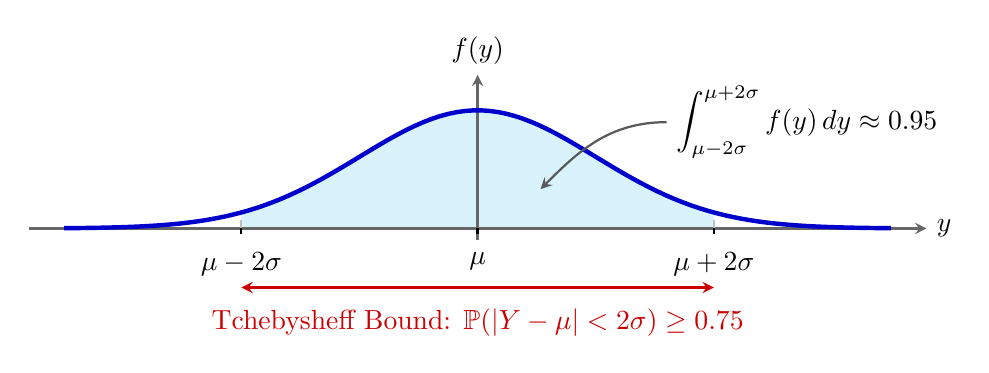
\begin{tikzpicture}[
    scale=1.5, % Natively expands canvas space to eliminate text collisions
    >=stealth
]
    % 1. LAYER 1: Background Shading (Executed first)
    \fill[fill=cyan!15] (-2,0) -- plot[domain=-2:2, samples=60] (\x, {exp(-0.5*\x*\x)}) -- (2,0) -- cycle;
    
    % 2. LAYER 2: Clean Axes (Slightly extended past curve tails)
    \draw[->, thick, gray!80!black] (-3.8, 0) -- (3.8, 0) node[right, black] {$y$};
    \draw[->, thick, gray!80!black] (0, -0.1) -- (0, 1.3) node[above, black] {$f(y)$};
    
    % 3. LAYER 3: Boundary Indicators & Primary Plot Curve
    \draw[dashed, thick, gray!50] (-2,0) -- (-2, {exp(-0.5*(-2)*(-2))});
    \draw[dashed, thick, gray!50] (2,0) -- (2, {exp(-0.5*2*2)});
    \draw[ultra thick, blue!80!black, domain=-3.5:3.5, samples=100] plot (\x, {exp(-0.5*\x*\x)});
    
    % 4. LAYER 4: Decoupled Axis Ticks & Alignment Labels
    \draw[thick] (0,0) -- (0,-0.05) node[below=3pt, black] {$\mu$};
    \draw[thick] (-2,0) -- (-2,-0.05) node[below=3pt, black] {$\mu - 2\sigma$};
    \draw[thick] (2,0) -- (2,-0.05) node[below=3pt, black] {$\mu + 2\sigma$};

    % 5. LAYER 5: Off-Axis Formula Callout (The "Off-Axis" Rule)
    % Moves the integral completely clear of the hump using a soft indicator line
    \coordinate (ShadedRegion) at (0.5, 0.3);
    \node[anchor=west, black] (AreaEq) at (1.6, 0.9) {$\displaystyle \int_{\mu-2\sigma}^{\mu+2\sigma} f(y) \, dy \approx 0.95$};
    \draw[->, shorten >=2pt, thick, gray!70!black] (AreaEq.west) to[out=180, in=45] (ShadedRegion);

    % 6. LAYER 6: Tchebysheff Bound Interval Representation
    % Separates the horizontal span indicator from the text line to stop overcrowding
    \draw[<->, thick, red!80!black] (-2, -0.5) -- (2, -0.5);
    \node[below=4pt, red!80!black] at (0, -0.5) {Tchebysheff Bound: $\mathbb{P}(|Y - \mu| < 2\sigma) \ge 0.75$};

\end{tikzpicture}
\end{center}


\subsection{Heuristics and "Cheats"}
\begin{itemize}
    \item \textbf{The $t=0$ Sanity Check:} For any valid MGF, $m(0)$ MUST equal $1$. If you derive an MGF and $m(0) \neq 1$, your integration is incorrect.
    \item \textbf{Linearity Shortcut:} If you know the MGF of $Z \sim N(0,1)$ is $e^{t^2/2}$, you can instantly find the MGF of $X \sim N(\mu, \sigma^2)$ by writing $X = \sigma Z + \mu$ and applying the linear transformation rule: $m_X(t) = e^{\mu t} m_Z(\sigma t) = e^{\mu t + \sigma^2 t^2 / 2}$.
\end{itemize}

\subsection{Pitfalls and Fallacies}
\begin{itemize}
    \item \textbf{The Existence Fallacy:} Assuming every random variable has an MGF. Heavy-tailed distributions (like the Cauchy or Lognormal distributions) do not have MGFs because the integral $\E[e^{tY}]$ diverges to infinity for $t > 0$.
    \item \textbf{The Exactness Fallacy:} Treating Tchebysheff's bound as an exact probability. Tchebysheff provides a \textit{worst-case scenario} bound. As seen in Problem 4.149, the actual probability can be much higher (e.g., $1.00$ vs the bound of $0.75$).
\end{itemize}

\newpage

\section{Part 5: Conceptual Synthesis and The "Big Picture"}

\subsection{A) Thematic Connections}
The central theme unifying this chapter is the concept of \textbf{Integral Transforms as Analytical Bridges}. In mathematics, when a problem is intractable in its native space (the spatial/time domain), we transform it into a dual space (the frequency domain) where the operations become trivial. 
Just as logarithms turn multiplication into addition, the Moment-Generating Function (a real-valued Laplace transform) turns the complex convolution of probability density functions into simple algebraic multiplication. If $X$ and $Y$ are independent, the PDF of $X+Y$ is $f_X * f_Y$ (a difficult integral), but their MGF is simply $m_{X+Y}(t) = m_X(t)m_Y(t)$.

\subsection{B) Forward and Backward Links}
\textbf{Backwards:} This topic builds directly upon the Law of the Unconscious Statistician (LOTUS), which justifies computing $\E[g(Y)]$ using the PDF of $Y$ without needing to find the PDF of $g(Y)$ first. Here, $g(Y) = e^{tY}$.
\textbf{Forwards:} The MGF is the necessary stepping stone to the \textbf{Characteristic Function}, defined as $\phi_Y(t) = \E[e^{itY}]$ where $i = \sqrt{-1}$. Because $|e^{itY}| = 1$, the characteristic function is guaranteed to exist for \textit{all} probability distributions, solving the "Existence Fallacy" of MGFs. Furthermore, the algebraic properties of MGFs/Characteristic Functions form the rigorous bedrock for proving the \textbf{Central Limit Theorem} via Levy's Continuity Theorem.

\section{Part 6: Abstract Real-World Modeling (AI, ML, \& Quant Finance)}

\subsection{A) Concrete Scenarios}
\begin{enumerate}
    \item \textbf{Algorithmic Trading (Risk Management):} When quantitative hedge funds model the returns of exotic assets, the true underlying probability distribution is often unknown and highly non-normal. Tchebysheff's inequality is used to establish distribution-free Value at Risk (VaR) bounds, ensuring that the probability of a catastrophic portfolio loss is strictly bounded regardless of market dynamics.
    \item \textbf{Statistical Learning Theory (AI/ML):} In Machine Learning, we must guarantee that a model trained on finite data will generalize to unseen data. MGFs are the foundational tool used to prove \textbf{Hoeffding's Inequality} and \textbf{Chernoff Bounds}, which provide the PAC (Probably Approximately Correct) learning bounds that dictate the sample complexity required to train neural networks.
    \item \textbf{Quantitative Finance (Derivatives Pricing):} In advanced stochastic calculus, assets are modeled using affine jump-diffusion models (e.g., the Heston Model). The SDEs governing these models are too complex to yield closed-form PDFs. However, their MGFs can be solved analytically. Options are then priced by evaluating the MGF in the complex plane and using Fourier inversion techniques (the Carr-Madan formula).
\end{enumerate}

\subsection{B) Model Problem Setup: PAC Learning Bounds in AI}
Let us construct a rigorous mathematical model for bounding generalization error in Machine Learning using concepts derived from MGFs.

\textbf{State Space and Random Variables:} Let $\mathcal{X} \subset \R^d$ be the feature space and $\mathcal{Y} = \{0, 1\}$ be the label space. Let $Z_i = (X_i, Y_i)$ for $i = 1, \dots, n$ be a sequence of training samples drawn independent and identically distributed (i.i.d.) from an unknown, true probability measure $\Prob$ over $\mathcal{X} \times \mathcal{Y}$.

\textbf{Hypothesis and Loss Function:} Let $h: \mathcal{X} \to \mathcal{Y}$ be a neural network classifier. We define a 0-1 loss function $\ell(h(X), Y) \in [0, 1]$. 
The \textit{True Risk} (expected out-of-sample error) is $L(h) = \E_{\Prob}[\ell(h(X), Y)]$.
The \textit{Empirical Risk} (in-sample training error) is $\hat{L}(h) = \frac{1}{n} \sum_{i=1}^n \ell(h(X_i), Y_i)$.

\textbf{The Optimization Constraint:} We must bound the probability that the empirical risk deviates from the true risk by more than a tolerance $\epsilon > 0$. Using Chernoff bounds (which are derived directly from optimizing the MGF of the loss random variables), we obtain Hoeffding's Inequality:
\[ \Prob\left( |\hat{L}(h) - L(h)| \ge \epsilon \right) \le 2 \exp(-2n\epsilon^2) \]
This inequality allows AI researchers to mathematically guarantee that as the number of training samples $n \to \infty$, the probability of the model failing to generalize decays exponentially fast.

\newpage

\section{Part 7: Common Variations and Untested Concepts}

A critical concept taught in advanced probability courses, which extends Tchebysheff's Theorem, is the \textbf{Chernoff Bound}. While Tchebysheff provides a polynomial tail bound ($1/k^2$) using only the variance, the Chernoff bound utilizes the entire MGF to provide a much tighter, exponential tail bound.

\begin{theorem}[The Chernoff Bound]
For any random variable $Y$ with MGF $m_Y(t)$, and for any real number $a$:
\[ \Prob(Y \ge a) \le \inf_{t > 0} e^{-ta} m_Y(t) \]
\end{theorem}

\textbf{Rigorous Proof:}
Let $t > 0$. Because the exponential function $g(y) = e^{ty}$ is strictly monotonically increasing, the event $\{Y \ge a\}$ is logically and set-theoretically identical to the event $\{e^{tY} \ge e^{ta}\}$. Therefore, their probability measures must be equal:
\[ \Prob(Y \ge a) = \Prob(e^{tY} \ge e^{ta}) \]
Notice that $X = e^{tY}$ is a strictly non-negative random variable. We can apply Markov's Inequality ($\Prob(X \ge c) \le \E[X]/c$):
\[ \Prob(e^{tY} \ge e^{ta}) \le \frac{\E[e^{tY}]}{e^{ta}} \]
By the definition of the Moment-Generating Function, $\E[e^{tY}] = m_Y(t)$. Substituting this yields:
\[ \Prob(Y \ge a) \le e^{-ta} m_Y(t) \]
Because this inequality holds true for \textit{any} choice of $t > 0$, we can find the tightest possible bound by taking the infimum over all $t > 0$:
\[ \Prob(Y \ge a) \le \inf_{t > 0} e^{-ta} m_Y(t) \]
$\blacksquare$

\section{Part 8: Advanced Diagnostic Testing: "Find the Flaw"}

Below are five advanced proofs containing subtle, critical flaws. 

\textbf{Problem 1:} Let $Y$ follow a standard Cauchy distribution with PDF $f(y) = \frac{1}{\pi(1+y^2)}$. To find the mean of $Y$, we first compute the MGF: $m_Y(t) = \int_{-\infty}^{\infty} e^{ty} \frac{1}{\pi(1+y^2)} dy$. Since the integrand is strictly positive, the integral evaluates to some function $M(t)$. We then find the mean by evaluating $M'(0)$.
\textit{Find the Flaw.}

\textbf{Problem 2:} A factory produces items with mean weight $\mu = 50$g and $\sigma = 5$g. We take a sample of $n=100$ items. By Tchebysheff's inequality, the probability that the sample mean $\bar{Y}$ deviates from $\mu$ by more than $2$g is bounded by: $\Prob(|\bar{Y} - \mu| \ge 2) = \Prob(|\bar{Y} - \mu| \ge 0.4\sigma) \le \frac{1}{0.4^2} = 6.25$.
\textit{Find the Flaw.}

\textbf{Problem 3:} Let $X$ and $Y$ be two random variables (not necessarily independent). The MGF of their sum $Z = X+Y$ is derived as follows: $m_Z(t) = \E[e^{t(X+Y)}] = \E[e^{tX} e^{tY}] = \E[e^{tX}] \E[e^{tY}] = m_X(t) m_Y(t)$.
\textit{Find the Flaw.}

\textbf{Problem 4:} Let $X$ and $Y$ be random variables. We compute their MGFs and find that $m_X(1) = 2$ and $m_Y(1) = 2$. Since their MGFs are equal at $t=1$, by the Uniqueness Theorem, $X$ and $Y$ must have the exact same probability distribution.
\textit{Find the Flaw.}

\textbf{Problem 5:} We wish to find the expected value of $1/X$. We know the MGF is $m_X(t) = \E[e^{tX}]$. If we evaluate the MGF at $t = -1$, we get $m_X(-1) = \E[e^{-X}] = \E[1/e^X]$. By Taylor expansion, this approximates $\E[1/X]$.
\textit{Find the Flaw.}

\vspace{0.5cm}
\hrule
\vspace{0.5cm}

\subsection{Solution Key: Resolutions to the Flaws}
\textbf{Resolution 1 (Existence of MGF):} The flaw is assuming the integral converges. For the Cauchy distribution, $e^{ty}$ grows exponentially in the numerator, while $(1+y^2)$ only grows quadratically in the denominator. The integral diverges to infinity for all $t \neq 0$. The MGF does not exist, and the Cauchy distribution has an undefined mean.

\textbf{Resolution 2 (Variance of Sample Mean \& Vacuous Bounds):} There are two flaws. First, the standard deviation of the sample mean $\bar{Y}$ is not $\sigma$, but the standard error $\sigma/\sqrt{n} = 5/10 = 0.5$. The correct $k$ is $2 / 0.5 = 4$, yielding a bound of $1/16$. Second, a probability bound of $6.25$ is mathematically vacuous since all probabilities must be $\le 1$.

\textbf{Resolution 3 (Independence Assumption):} The step $\E[e^{tX} e^{tY}] = \E[e^{tX}] \E[e^{tY}]$ is a severe logical fallacy. The expectation of a product only equals the product of expectations if the random variables $e^{tX}$ and $e^{tY}$ are uncorrelated, which generally requires $X$ and $Y$ to be strictly independent.

\textbf{Resolution 4 (Uniqueness Theorem Conditions):} The Uniqueness Theorem requires $m_X(t) = m_Y(t)$ for all $t$ in an \textit{open interval} $(-b, b)$ containing zero. Equality at a single, isolated non-zero point ($t=1$) is entirely insufficient to prove the distributions are identical.

\textbf{Resolution 5 (LOTUS Violation):} The flaw is confusing the functions. $\E[e^{-X}]$ is strictly the expected value of the function $g(x) = e^{-x}$. This is fundamentally different from the expected value of $h(x) = 1/x$. You cannot use the MGF to directly compute $\E[1/X]$.

\end{document}